\chapter{Grafs dirigits}

En aquest capítol, ens centrem en dues classes de grafs dirigits:
\begin{itemize}
\item \key{Acyclic graphs}:
There are no cycles in the graph,
so there is no path from any node to itself\footnote{Directed acyclic
graphs are sometimes called DAGs.}.
\item \key{Successor graphs}:
The outdegree of each node is 1,
so each node has a unique successor.
\end{itemize}
Resulta que en ambdós casos podem dissenyar algorismes eficients que
es basen en propietats especials dels grafs.

\section{Ordenació topològica}

\index{ordenació topològica} \index{cicle}

Una \key{ordenació topològica} és una ordenació dels nodes d'un graf
dirigit de manera que quan hi ha un camí des del node $a$ fins al node
$b$ es complex que el node $a$ apareix abans que el node $b$ en
l'ordenació. Per exemple, per al graf
\begin{center}
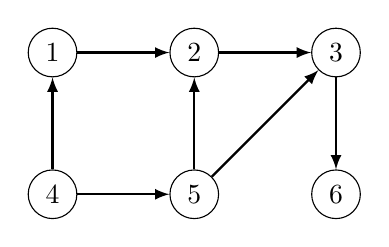
\begin{tikzpicture}[scale=0.9]
\node[draw, circle] (1) at (1,5) {$1$};
\node[draw, circle] (2) at (3,5) {$2$};
\node[draw, circle] (3) at (5,5) {$3$};
\node[draw, circle] (4) at (1,3) {$4$};
\node[draw, circle] (5) at (3,3) {$5$};
\node[draw, circle] (6) at (5,3) {$6$};

\path[draw,thick,->,>=latex] (1) -- (2);
\path[draw,thick,->,>=latex] (2) -- (3);
\path[draw,thick,->,>=latex] (4) -- (1);
\path[draw,thick,->,>=latex] (4) -- (5);
\path[draw,thick,->,>=latex] (5) -- (2);
\path[draw,thick,->,>=latex] (5) -- (3);
\path[draw,thick,->,>=latex] (3) -- (6);
\end{tikzpicture}
\end{center}
es té que $[4,1,5,2,3,6]$ és una possible ordenació topològica:
\begin{center}
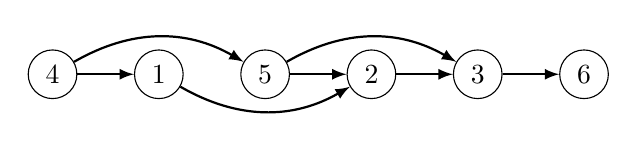
\begin{tikzpicture}[scale=0.9]
\node[draw, circle] (1) at (-6,0) {$1$};
\node[draw, circle] (2) at (-3,0) {$2$};
\node[draw, circle] (3) at (-1.5,0) {$3$};
\node[draw, circle] (4) at (-7.5,0) {$4$};
\node[draw, circle] (5) at (-4.5,0) {$5$};
\node[draw, circle] (6) at (-0,0) {$6$};

\path[draw,thick,->,>=latex] (1) edge [bend right=30] (2);
\path[draw,thick,->,>=latex] (2) -- (3);
\path[draw,thick,->,>=latex] (4) -- (1);
\path[draw,thick,->,>=latex] (4) edge [bend left=30] (5);
\path[draw,thick,->,>=latex] (5) -- (2);
\path[draw,thick,->,>=latex] (5) edge [bend left=30]  (3);
\path[draw,thick,->,>=latex] (3) -- (6);
\end{tikzpicture}
\end{center}


Un graf acíclic sempre té una ordenació topològica. Tanmateix, si el
graf conté un cicle, no és possible formar una ordenació topològica,
perquè cap node del cicle pot aparèixer abans que els altres nodes del
cicle en l'ordenació. Resulta que la cerca en profunditat es pot
fer servir tant per comprovar si un graf dirigit conté un cicle com, si
no conté un cicle, per construir una ordenació topològica.

\subsubsection{Algorisme}

La idea és iterar tots els nodes del graf, iniciant una nova cerca en
profunditat cada cop que trobem un node sence processar. Durant el
recorregut, els nodes poden tenir tres estats possibles:


\begin{itemize}
\item state 0: the node has not been processed (white)
\item state 1: the node is under processing (light gray)
\item state 2: the node has been processed (dark gray)
\end{itemize}


Inicialment, l'estat de cada node és 0. Quan una cerca arriba a un
node per primera vegada, el seu estat passa a ser 1. Un cop hem
processat tots els els successors del node, el seu estat passa a ser
2.

Si el graf conté un cicle, ho descobrirem durant la cerca, perquè tard
o d'hora arribarem a un node l'estat del qual és 1. En aquest cas, no
és possible construir un ordenament topològic.

Si el graf no conté cap cicle, podem construir una ordenació
topològica afegint cada node a una llista quan l'estat del node esdevé
2. Aquesta llista conté una ordenació topològica en ordre invers.

\subsubsection{Exemple 1}

Al graf d'exemple, la cerca passa del node 1 al node 6:


\begin{center}
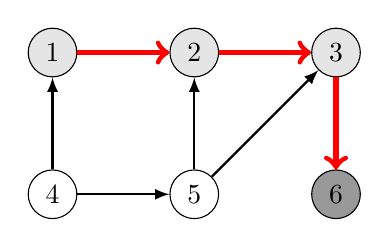
\begin{tikzpicture}[scale=0.9]
\node[draw, circle,fill=gray!20] (1) at (1,5) {$1$};
\node[draw, circle,fill=gray!20] (2) at (3,5) {$2$};
\node[draw, circle,fill=gray!20] (3) at (5,5) {$3$};
\node[draw, circle] (4) at (1,3) {$4$};
\node[draw, circle] (5) at (3,3) {$5$};
\node[draw, circle,fill=gray!80] (6) at (5,3) {$6$};

\path[draw,thick,->,>=latex] (4) -- (1);
\path[draw,thick,->,>=latex] (4) -- (5);
\path[draw,thick,->,>=latex] (5) -- (2);
\path[draw,thick,->,>=latex] (5) -- (3);
%\path[draw,thick,->,>=latex] (3) -- (6);

\path[draw=red,thick,->,line width=2pt] (1) -- (2);
\path[draw=red,thick,->,line width=2pt] (2) -- (3);
\path[draw=red,thick,->,line width=2pt] (3) -- (6);
\end{tikzpicture}
\end{center}


Amb això hem processat el node 6, de manera que l'afegim a la
llista. Després d'això, també afegim els nodes 3, 2 i 1 a la
llista:


\begin{center}
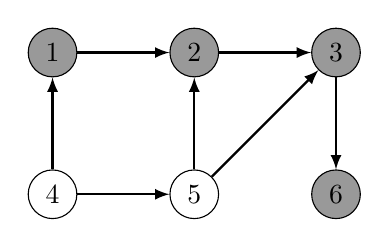
\begin{tikzpicture}[scale=0.9]
\node[draw, circle,fill=gray!80] (1) at (1,5) {$1$};
\node[draw, circle,fill=gray!80] (2) at (3,5) {$2$};
\node[draw, circle,fill=gray!80] (3) at (5,5) {$3$};
\node[draw, circle] (4) at (1,3) {$4$};
\node[draw, circle] (5) at (3,3) {$5$};
\node[draw, circle,fill=gray!80] (6) at (5,3) {$6$};

\path[draw,thick,->,>=latex] (1) -- (2);
\path[draw,thick,->,>=latex] (2) -- (3);
\path[draw,thick,->,>=latex] (4) -- (1);
\path[draw,thick,->,>=latex] (4) -- (5);
\path[draw,thick,->,>=latex] (5) -- (2);
\path[draw,thick,->,>=latex] (5) -- (3);
\path[draw,thick,->,>=latex] (3) -- (6);
\end{tikzpicture}
\end{center}


En aquest punt, la llista és $[6,3,2,1]$. La cerca següent comença al
node 4:


\begin{center}
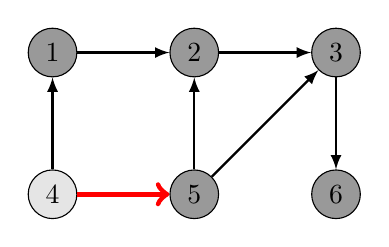
\begin{tikzpicture}[scale=0.9]
\node[draw, circle,fill=gray!80] (1) at (1,5) {$1$};
\node[draw, circle,fill=gray!80] (2) at (3,5) {$2$};
\node[draw, circle,fill=gray!80] (3) at (5,5) {$3$};
\node[draw, circle,fill=gray!20] (4) at (1,3) {$4$};
\node[draw, circle,fill=gray!80] (5) at (3,3) {$5$};
\node[draw, circle,fill=gray!80] (6) at (5,3) {$6$};

\path[draw,thick,->,>=latex] (1) -- (2);
\path[draw,thick,->,>=latex] (2) -- (3);
\path[draw,thick,->,>=latex] (4) -- (1);
%\path[draw,thick,->,>=latex] (4) -- (5);
\path[draw,thick,->,>=latex] (5) -- (2);
\path[draw,thick,->,>=latex] (5) -- (3);
\path[draw,thick,->,>=latex] (3) -- (6);

\path[draw=red,thick,->,line width=2pt] (4) -- (5);
\end{tikzpicture}
\end{center}


Així, la llista final és $[6,3,2,1,5,4]$. Hem processat tots els
nodes, de manera que hem trobat una ordenació classificació
topològica, la llista inversa $[4,5,1,2,3,6]$:


\begin{center}
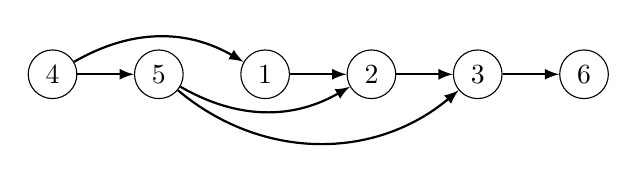
\begin{tikzpicture}[scale=0.9]
\node[draw, circle] (1) at (3,0) {$1$};
\node[draw, circle] (2) at (4.5,0) {$2$};
\node[draw, circle] (3) at (6,0) {$3$};
\node[draw, circle] (4) at (0,0) {$4$};
\node[draw, circle] (5) at (1.5,0) {$5$};
\node[draw, circle] (6) at (7.5,0) {$6$};

\path[draw,thick,->,>=latex] (1) -- (2);
\path[draw,thick,->,>=latex] (2) -- (3);
\path[draw,thick,->,>=latex] (4) edge [bend left=30] (1);
\path[draw,thick,->,>=latex] (4) -- (5);
\path[draw,thick,->,>=latex] (5) edge [bend right=30] (2);
\path[draw,thick,->,>=latex] (5) edge [bend right=40] (3);
\path[draw,thick,->,>=latex] (3) -- (6);
\end{tikzpicture}
\end{center}


Tingueu en compte que les ordenacions topològiques no són úniques, i que per tant, un
graf donat pot tenir moltes ordenacions topològiques distintes.

\subsubsection{Exemple 2}

Considerem ara un graf per al qual no podem construir cap ordenació
topològica, perquè el graf conté un cicle:


\begin{center}
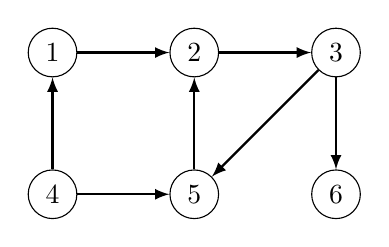
\begin{tikzpicture}[scale=0.9]
\node[draw, circle] (1) at (1,5) {$1$};
\node[draw, circle] (2) at (3,5) {$2$};
\node[draw, circle] (3) at (5,5) {$3$};
\node[draw, circle] (4) at (1,3) {$4$};
\node[draw, circle] (5) at (3,3) {$5$};
\node[draw, circle] (6) at (5,3) {$6$};

\path[draw,thick,->,>=latex] (1) -- (2);
\path[draw,thick,->,>=latex] (2) -- (3);
\path[draw,thick,->,>=latex] (4) -- (1);
\path[draw,thick,->,>=latex] (4) -- (5);
\path[draw,thick,->,>=latex] (5) -- (2);
\path[draw,thick,->,>=latex] (3) -- (5);
\path[draw,thick,->,>=latex] (3) -- (6);
\end{tikzpicture}
\end{center}
La cerca continua de la següent manera:
\begin{center}
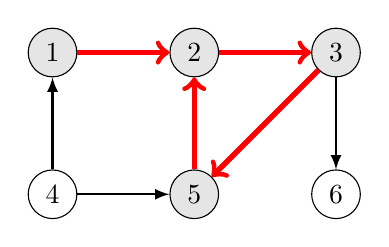
\begin{tikzpicture}[scale=0.9]
\node[draw, circle,fill=gray!20] (1) at (1,5) {$1$};
\node[draw, circle,fill=gray!20] (2) at (3,5) {$2$};
\node[draw, circle,fill=gray!20] (3) at (5,5) {$3$};
\node[draw, circle] (4) at (1,3) {$4$};
\node[draw, circle,fill=gray!20] (5) at (3,3) {$5$};
\node[draw, circle] (6) at (5,3) {$6$};

\path[draw,thick,->,>=latex] (4) -- (1);
\path[draw,thick,->,>=latex] (4) -- (5);
\path[draw,thick,->,>=latex] (3) -- (6);

\path[draw=red,thick,->,line width=2pt] (1) -- (2);
\path[draw=red,thick,->,line width=2pt] (2) -- (3);
\path[draw=red,thick,->,line width=2pt] (3) -- (5);
\path[draw=red,thick,->,line width=2pt] (5) -- (2);
\end{tikzpicture}
\end{center}
La cerca arriba al node 2 l'estat del qual és 1, el que significa que
el graf conté un cicle. En aquest exemple, hi ha un cicle $2
\rightarrow 3 \rightarrow 5 \rightarrow 2$.

\section{Programació dinàmica}

Quan un graf dirigit és acíclic podem aplicar-hi programació
dinàmica. Per exemple, podem resoldre de manera eficient els problemes
següents relacionats amb els camins des d'un node inicial fins a un
node final:


\begin{itemize}
\item how many different paths are there?
\item what is the shortest/longest path?
\item what is the minimum/maximum number of edges in a path?
\item which nodes certainly appear in any path?
\end{itemize}


\subsubsection{Comptar el nombre de camins}

Per exemple, calculem el nombre de camins del node 1 al node 6 en el
graf següent:


\begin{center}
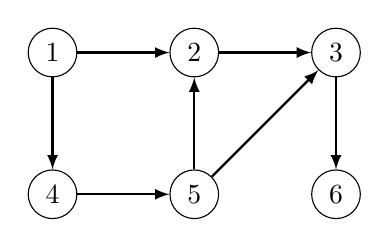
\begin{tikzpicture}[scale=0.9]
\node[draw, circle] (1) at (1,5) {$1$};
\node[draw, circle] (2) at (3,5) {$2$};
\node[draw, circle] (3) at (5,5) {$3$};
\node[draw, circle] (4) at (1,3) {$4$};
\node[draw, circle] (5) at (3,3) {$5$};
\node[draw, circle] (6) at (5,3) {$6$};

\path[draw,thick,->,>=latex] (1) -- (2);
\path[draw,thick,->,>=latex] (2) -- (3);
\path[draw,thick,->,>=latex] (1) -- (4);
\path[draw,thick,->,>=latex] (4) -- (5);
\path[draw,thick,->,>=latex] (5) -- (2);
\path[draw,thick,->,>=latex] (5) -- (3);
\path[draw,thick,->,>=latex] (3) -- (6);
\end{tikzpicture}
\end{center}
Hi ha un total de tres camins d'aquest tipus:
\begin{itemize}
\item $1 \rightarrow 2 \rightarrow 3 \rightarrow 6$
\item $1 \rightarrow 4 \rightarrow 5 \rightarrow 2 \rightarrow 3 \rightarrow 6$
\item $1 \rightarrow 4 \rightarrow 5 \rightarrow 3 \rightarrow 6$
\end{itemize}


Sigui $\texttt{paths}(x)$ el nombre de camins des del node 1 fins al
node $x$. Com a cas base, $\texttt{camins}(1)=1$. Podem calcular els valors de
$\texttt{camins}(x)$ fent servir la recursió
\[\texttt{paths}(x) = \texttt{paths}(a_1)+\texttt{paths}(a_2)+\cdots+\texttt{paths}(a_k)\]
on $a_1,a_2,\ldots,a_k$ són els nodes dels quals surt una aresta cap a
$x$. Com que el graf és acíclic, una ordenació topològica ens permet calcular els
valors de $\texttt{paths}(x)$ amb programació dinàmica. Per exemple, aquesta és
una ordenació topològica del graf:
\begin{center}
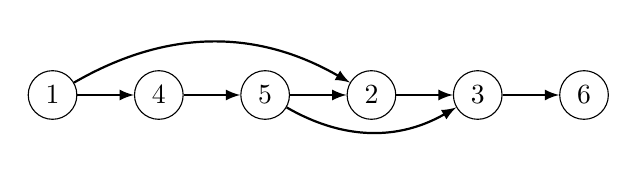
\begin{tikzpicture}[scale=0.9]
\node[draw, circle] (1) at (0,0) {$1$};
\node[draw, circle] (2) at (4.5,0) {$2$};
\node[draw, circle] (3) at (6,0) {$3$};
\node[draw, circle] (4) at (1.5,0) {$4$};
\node[draw, circle] (5) at (3,0) {$5$};
\node[draw, circle] (6) at (7.5,0) {$6$};

\path[draw,thick,->,>=latex] (1) edge [bend left=30] (2);
\path[draw,thick,->,>=latex] (2) -- (3);
\path[draw,thick,->,>=latex] (1) -- (4);
\path[draw,thick,->,>=latex] (4) -- (5);
\path[draw,thick,->,>=latex] (5) -- (2);
\path[draw,thick,->,>=latex] (5) edge [bend right=30] (3);
\path[draw,thick,->,>=latex] (3) -- (6);
\end{tikzpicture}
\end{center}
Per tant, els nombres de camins són:
\begin{center}
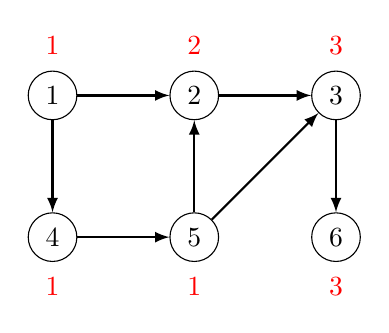
\begin{tikzpicture}[scale=0.9]
\node[draw, circle] (1) at (1,5) {$1$};
\node[draw, circle] (2) at (3,5) {$2$};
\node[draw, circle] (3) at (5,5) {$3$};
\node[draw, circle] (4) at (1,3) {$4$};
\node[draw, circle] (5) at (3,3) {$5$};
\node[draw, circle] (6) at (5,3) {$6$};

\path[draw,thick,->,>=latex] (1) -- (2);
\path[draw,thick,->,>=latex] (2) -- (3);
\path[draw,thick,->,>=latex] (1) -- (4);
\path[draw,thick,->,>=latex] (4) -- (5);
\path[draw,thick,->,>=latex] (5) -- (2);
\path[draw,thick,->,>=latex] (5) -- (3);
\path[draw,thick,->,>=latex] (3) -- (6);

\node[color=red] at (1,2.3) {$1$};
\node[color=red] at (3,2.3) {$1$};
\node[color=red] at (5,2.3) {$3$};
\node[color=red] at (1,5.7) {$1$};
\node[color=red] at (3,5.7) {$2$};
\node[color=red] at (5,5.7) {$3$};
\end{tikzpicture}
\end{center}


Per exemple, per calcular el valor de $\texttt{paths}(3)$, fem servir
la fórmula $\texttt{paths}(2)+\texttt{paths}(5)$, perquè hi ha arestes
que surten dels nodes 2 i 5 al node 3. Com que $\texttt{paths}(2)=2$ i
$\texttt{paths}(5)=1$, concloem que $\texttt{paths}(3)=3$.

\subsubsection{Extensió de l'algorisme de Dijkstra}

\index{Algorisme de Dijkstra}

Un subproducte de l'algorisme de Dijkstra és un graf acíclic dirigit
que indica per a cada node del graf original les possibles maneres
d'arribar al node des del node inicial fent servir camins mínims.
Podem aplicar programació dinàmica en aquest graf. Per exemple, en el
graf
\begin{center}
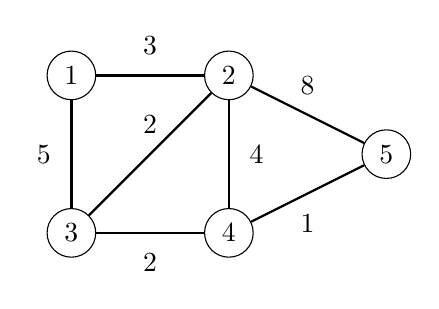
\begin{tikzpicture}
\node[draw, circle] (1) at (0,0) {$1$};
\node[draw, circle] (2) at (2,0) {$2$};
\node[draw, circle] (3) at (0,-2) {$3$};
\node[draw, circle] (4) at (2,-2) {$4$};
\node[draw, circle] (5) at (4,-1) {$5$};

\path[draw,thick,-] (1) -- node[font=\small,label=above:3] {} (2);
\path[draw,thick,-] (1) -- node[font=\small,label=left:5] {} (3);
\path[draw,thick,-] (2) -- node[font=\small,label=right:4] {} (4);
\path[draw,thick,-] (2) -- node[font=\small,label=above:8] {} (5);
\path[draw,thick,-] (3) -- node[font=\small,label=below:2] {} (4);
\path[draw,thick,-] (4) -- node[font=\small,label=below:1] {} (5);
\path[draw,thick,-] (2) -- node[font=\small,label=above:2] {} (3);
\end{tikzpicture}
\end{center}
els camins mínims des del node 1 poden fer servir les arestes següents:
\begin{center}
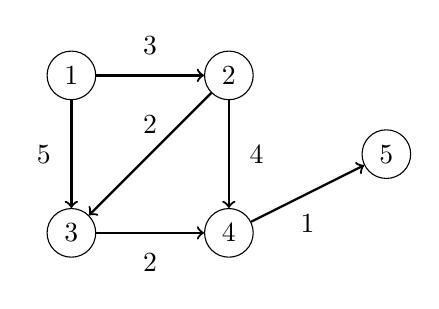
\begin{tikzpicture}
\node[draw, circle] (1) at (0,0) {$1$};
\node[draw, circle] (2) at (2,0) {$2$};
\node[draw, circle] (3) at (0,-2) {$3$};
\node[draw, circle] (4) at (2,-2) {$4$};
\node[draw, circle] (5) at (4,-1) {$5$};

\path[draw,thick,->] (1) -- node[font=\small,label=above:3] {} (2);
\path[draw,thick,->] (1) -- node[font=\small,label=left:5] {} (3);
\path[draw,thick,->] (2) -- node[font=\small,label=right:4] {} (4);
\path[draw,thick,->] (3) -- node[font=\small,label=below:2] {} (4);
\path[draw,thick,->] (4) -- node[font=\small,label=below:1] {} (5);
\path[draw,thick,->] (2) -- node[font=\small,label=above:2] {} (3);
\end{tikzpicture}
\end{center}


Ara podem, per exemple, calcular el nombre de camins mínims del
node 1 al node 5 mitjançant la programació dinàmica:
\begin{center}
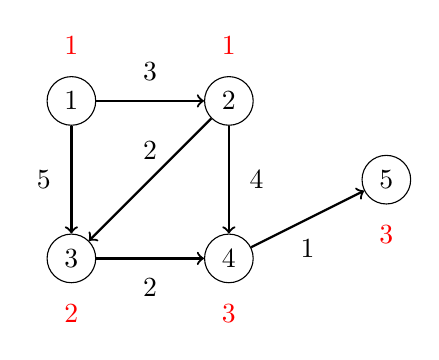
\begin{tikzpicture}
\node[draw, circle] (1) at (0,0) {$1$};
\node[draw, circle] (2) at (2,0) {$2$};
\node[draw, circle] (3) at (0,-2) {$3$};
\node[draw, circle] (4) at (2,-2) {$4$};
\node[draw, circle] (5) at (4,-1) {$5$};

\path[draw,thick,->] (1) -- node[font=\small,label=above:3] {} (2);
\path[draw,thick,->] (1) -- node[font=\small,label=left:5] {} (3);
\path[draw,thick,->] (2) -- node[font=\small,label=right:4] {} (4);
\path[draw,thick,->] (3) -- node[font=\small,label=below:2] {} (4);
\path[draw,thick,->] (4) -- node[font=\small,label=below:1] {} (5);
\path[draw,thick,->] (2) -- node[font=\small,label=above:2] {} (3);

\node[color=red] at (0,0.7) {$1$};
\node[color=red] at (2,0.7) {$1$};
\node[color=red] at (0,-2.7) {$2$};
\node[color=red] at (2,-2.7) {$3$};
\node[color=red] at (4,-1.7) {$3$};
\end{tikzpicture}
\end{center}


\subsubsection{Representació problemes com a grafs}

De fet, qualsevol problema de programació dinàmica es pot representar
com un graf acíclic dirigit. En aquest graf, cada node correspon a un
estat de la programació dinàmica, i les arestes indiquen que un estat
depèn d'un altre.

Per exemple, considereu el problema de formar una suma de diners $n$
fent servir monedes $\{c_1,c_2,\ldots,c_k\}$. En aquest problema, podem
construir un graf on cada node es correspon amb una suma de diners, i
les arestes mostren com triar una moneda. Per exemple, per a les
monedes $\{1,3,4\}$ i $n=6$, el graf és el següent:
\begin{center}
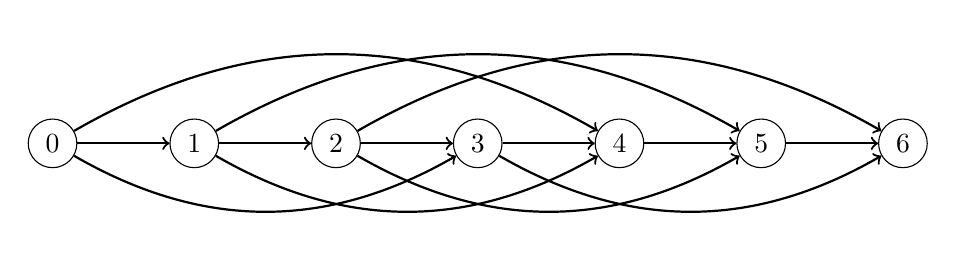
\begin{tikzpicture}[scale=0.9]
\node[draw, circle] (0) at (0,0) {$0$};
\node[draw, circle] (1) at (2,0) {$1$};
\node[draw, circle] (2) at (4,0) {$2$};
\node[draw, circle] (3) at (6,0) {$3$};
\node[draw, circle] (4) at (8,0) {$4$};
\node[draw, circle] (5) at (10,0) {$5$};
\node[draw, circle] (6) at (12,0) {$6$};

\path[draw,thick,->] (0) -- (1);
\path[draw,thick,->] (1) -- (2);
\path[draw,thick,->] (2) -- (3);
\path[draw,thick,->] (3) -- (4);
\path[draw,thick,->] (4) -- (5);
\path[draw,thick,->] (5) -- (6);

\path[draw,thick,->] (0) edge [bend right=30] (3);
\path[draw,thick,->] (1) edge [bend right=30] (4);
\path[draw,thick,->] (2) edge [bend right=30] (5);
\path[draw,thick,->] (3) edge [bend right=30] (6);

\path[draw,thick,->] (0) edge [bend left=30] (4);
\path[draw,thick,->] (1) edge [bend left=30] (5);
\path[draw,thick,->] (2) edge [bend left=30] (6);
\end{tikzpicture}
\end{center}


Utilitzant aquesta representació, el camí mínim del node 0 al node $n$
es correspon amb una solució que fa servir el nombre mínim de monedes,
i el nombre total de camins des del node 0 al node $n$ és igual al
nombre total de solucions.

\section{Camins de successió}

\index{graf de successió} \index{graf funcional}
\label{camins-de-successio}

Per a la resta del capítol, ens centrarem en \key{grafs
 de successió}. En aquests grafs, el grau de sortida de cada node és 1,
és a dir, exactament una aresta comença en cada node. Un graf
successor consta d'un o més components, cadascun dels quals conté un
cicle i alguns camins que van a parar al cicle.

Els grafs de successió de vegades s'anomenen \key{grafs
  funcionals}. La raó d'això és que qualsevol graf de successió es
correspon amb una funció que defineix les arestes del graf. El
paràmetre de la funció és un node del graf i la funció retorna el
successor d'aquest node.

Per exemple, la funció
\begin{center}
\begin{tabular}{r|rrrrrrrrr}
$x$ & 1 & 2 & 3 & 4 & 5 & 6 & 7 & 8 & 9 \\
\hline
$\texttt{succ}(x)$ & 3 & 5 & 7 & 6 & 2 & 2 & 1 & 6 & 3 \\
\end{tabular}
\end{center}
defineix el següent graf:
\begin{center}
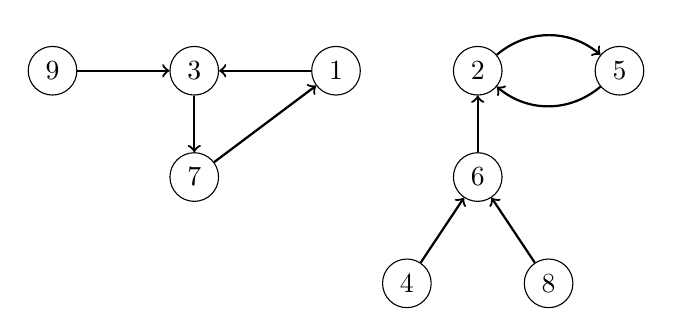
\begin{tikzpicture}[scale=0.9]
\node[draw, circle] (1) at (0,0) {$1$};
\node[draw, circle] (2) at (2,0) {$2$};
\node[draw, circle] (3) at (-2,0) {$3$};
\node[draw, circle] (4) at (1,-3) {$4$};
\node[draw, circle] (5) at (4,0) {$5$};
\node[draw, circle] (6) at (2,-1.5) {$6$};
\node[draw, circle] (7) at (-2,-1.5) {$7$};
\node[draw, circle] (8) at (3,-3) {$8$};
\node[draw, circle] (9) at (-4,0) {$9$};

\path[draw,thick,->] (1) -- (3);
\path[draw,thick,->] (2)  edge [bend left=40] (5);
\path[draw,thick,->] (3) -- (7);
\path[draw,thick,->] (4) -- (6);
\path[draw,thick,->] (5)  edge [bend left=40] (2);
\path[draw,thick,->] (6) -- (2);
\path[draw,thick,->] (7) -- (1);
\path[draw,thick,->] (8) -- (6);
\path[draw,thick,->] (9) -- (3);
\end{tikzpicture}
\end{center}


Com que cada node d'un graf de successió té un únic successor, també
podem definir una funció $\texttt{succ}(x,k)$ que ens retorna el node al
qual arribarem si comencem pel node $x$ i avancem $k$ passos
endavant. Per exemple, al graf anterior $\texttt{succ}(4,6)=2$, perquè
arribarem al node 2 avançant 6 passos des del node 4:


\begin{center}
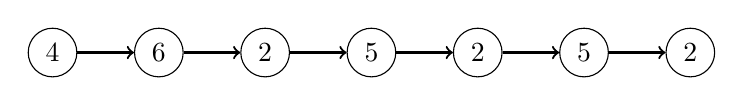
\begin{tikzpicture}[scale=0.9]
\node[draw, circle] (1) at (0,0) {$4$};
\node[draw, circle] (2) at (1.5,0) {$6$};
\node[draw, circle] (3) at (3,0) {$2$};
\node[draw, circle] (4) at (4.5,0) {$5$};
\node[draw, circle] (5) at (6,0) {$2$};
\node[draw, circle] (6) at (7.5,0) {$5$};
\node[draw, circle] (7) at (9,0) {$2$};

\path[draw,thick,->] (1) -- (2);
\path[draw,thick,->] (2) -- (3);
\path[draw,thick,->] (3) -- (4);
\path[draw,thick,->] (4) -- (5);
\path[draw,thick,->] (5) -- (6);
\path[draw,thick,->] (6) -- (7);
\end{tikzpicture}
\end{center}


Una manera senzilla de calcular el valor de $\texttt{succ}(x,k)$ és
començar al node $x$ i avançar $k$ passos endavant, i triga temps
$O(k)$. Tanmateix, fent servir preporcessament, qualsevol valor de
$\texttt{succ}(x,k)$ es pot calcular en temps $O(\log k)$.

La idea és precalcular tots els valors de $\texttt{succ}(x,k)$ on $k$
és una potència de dos i com a màxim $u$, on $u$ és el nombre màxim de
passos que permetem avançar. Això es pot fer de manera eficient fent
servir la següent recursió:


\begin{equation*}
    \texttt{succ}(x,k) = \begin{cases}
               \texttt{succ}(x)              & k = 1\\
               \texttt{succ}(\texttt{succ}(x,k/2),k/2)   & k > 1\\
           \end{cases}
\end{equation*}


Precalcular els valors requereix temps $O(n \log u)$, perquè hem de
calcular $O(\log u)$ valors per cada node. En el graf anterior, els
primers valors són els següents:


\begin{center}
\begin{tabular}{r|rrrrrrrrr}
$x$ & 1 & 2 & 3 & 4 & 5 & 6 & 7 & 8 & 9 \\
\hline
$\texttt{succ}(x,1)$ & 3 & 5 & 7 & 6 & 2 & 2 & 1 & 6 & 3 \\
$\texttt{succ}(x,2)$ & 7 & 2 & 1 & 2 & 5 & 5 & 3 & 2 & 7 \\
$\texttt{succ}(x,4)$ & 3 & 2 & 7 & 2 & 5 & 5 & 1 & 2 & 3 \\
$\texttt{succ}(x,8)$ & 7 & 2 & 1 & 2 & 5 & 5 & 3 & 2 & 7 \\
$\cdots$ \\
\end{tabular}
\end{center}


Després d'això, podem calcular qualsevol valor de $\texttt{succ}(x,k)$
representant el nombre de passos $k$ com una suma de potències de
dos. Per exemple, si volem calcular el valor de $\texttt{succ}(x,11)$,
primer formem la representació $11=8+2+1$. Amb això tenim
\[\texttt{succ}(x,11)=\texttt{succ}(\texttt{succ}(\texttt{succ}(x,8),2),1).\]
Per exemple, al graf anterior
\[\texttt{succ}(4,11)=\texttt{succ}(\texttt{succ}(\texttt{succ}(4,8),2),1)=5.\]


Aquesta representació sempre consta de $O(\log k)$ parts, de manera
que calcular un valor de $\texttt{succ}(x,k)$ triga temps $O(\log k)$.

\section{Detecció de cicles}

\index{cicle} \index{detecció de cicles}

Considereu un graf de successió que només conté un camí que acaba en
un cicle. Podem fer-nos les preguntes següents: si comencem la nostra
cerca al node inicial, quin és el primer node del cicle i quants
nodes conté el cicle?

Per exemple, en el graf


\begin{center}
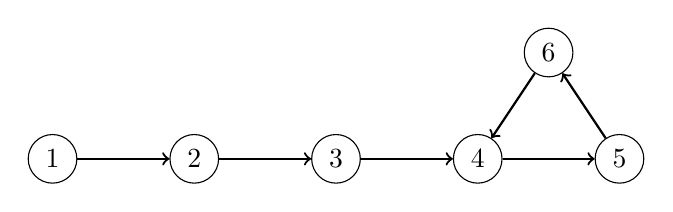
\begin{tikzpicture}[scale=0.9]
\node[draw, circle] (5) at (0,0) {$5$};
\node[draw, circle] (4) at (-2,0) {$4$};
\node[draw, circle] (6) at (-1,1.5) {$6$};
\node[draw, circle] (3) at (-4,0) {$3$};
\node[draw, circle] (2) at (-6,0) {$2$};
\node[draw, circle] (1) at (-8,0) {$1$};

\path[draw,thick,->] (1) -- (2);
\path[draw,thick,->] (2) -- (3);
\path[draw,thick,->] (3) -- (4);
\path[draw,thick,->] (4) -- (5);
\path[draw,thick,->] (5) -- (6);
\path[draw,thick,->] (6) -- (4);
\end{tikzpicture}
\end{center}
comencem el nostre camí al node 1, el primer node que pertany al cicle
és el node 4, i el cicle consta de tres nodes (4, 5 i 6).

Una manera senzilla de detectar el cicle és caminar pel graf i fer un
seguiment de tots els nodes que s'han visitat. Un cop visitat un node
per segona vegada, podem concloure que el node és el primer node del
cicle. Aquest mètode funciona en temps $O(n)$ i fa servir memòria
$O(n)$.

Tanmateix, hi ha millors algorismes per a la detecció de cicles. La
complexitat temporal d'aquests algorismes segueix sent $O(n)$, però
només fan servir memòria $O(1)$. Aquesta és una millora important si
$n$ és gran. A continuació parlarem de l'algorisme de Floyd que
compleix aquesta propietat.

\subsubsection{Algorisme de Floyd}

\index{Algorisme de Floyd}

L'\key{algorisme de Floyd}\footnote{La idea de l'algorisme s'esmenta a
\cite{knu982} i s'atribueix a R. W. Floyd; tanmateix, no se sap si
Floyd va descobrir realment l'algorisme.} avança pel graf fent servir
dos punters $a$ i $b$. Tots dos punters comencen en un node $x$ que és
el node inicial del graf. Aleshores, a cada pas, el punter $a$ fa un
pas endavant mentre que el punter $b$ fa dos passos endavant. El
procés continua fins que els punters es troben entre ells:
\begin{lstlisting}
a = succ(x);
b = succ(succ(x));
while (a != b) {
    a = succ(a);
    b = succ(succ(b));
}
\end{lstlisting}

A continuació, fem que el punter $a$ torni a apuntar a $x$, i avancem ambdós
punters pas a pas fins que es tornin a trobar. El punt on es tornen a trobar
és el primer node del cicle.
\begin{lstlisting}
a = x;
while (a != b) {
    a = succ(a);
    b = succ(b);
}
first = a;
\end{lstlisting}

La durada del cicle es calcula de la següent manera:
\begin{lstlisting}
b = succ(a);
length = 1;
while (a != b) {
    b = succ(b);
    length++;
}
\end{lstlisting}

Per què funciona l'algorisme de Floyd? Quan els punters $a$ i $b$ es
troben per primer cop, el punter $a$ ha fet $k$ passos i el punter $b$
ha fet $2k$ passos. El punter $b$ ha avançat $2k-k=k$ passos més que
el punter $a$, i com que aquests $k$ passos addicionals han estat
donant voltes de més al cicle, deduïm que la mida $c$ del cicle
divideix $k$. Sigui $k=v+w$, on $v$ és el nombre de passos que el
punter $a$ ha trigat a arribar al primer node del cicle i $w$ el
nombre de passos fets després. Amb aquesta notació, en la segona fase
de l'algorisme els punters $a$ i $b$ arribaran al primer node del
cicle en $v$ i $c-w$ passos respectivament. Però com que $c$ divideix
$k=v+w$, es compleix que $v+w=0$ mòdul $c$ o, equivalentment, $v =
c-w$ mòdul $c$. Aquesta congruència garanteix que en la segona fase de
l'algorisme els punters $a$ i $b$ es tornaran a trobar, i això només
pot passar en el primer node del cicle. Quan això passa, podem
calcular la mida $c$ del cicle fent que $b$ doni una volta de més,
fins retrobar $a$.
